\newpage
\section{Estimating Intrinsic Reward Functions}\label{appe:rewards}

In our approach, the intrinsic reward can be separated into two parts. One is related to action-aware diversity, while the other is related to observation-aware diversity. We revisit the formulation of our information-theoretic objective (Eq.~\ref{equ:per_timestep}) and discuss how to better estimate it.

\subsection{Intrinsic Rewards for Action-Aware Diversity}
\label{sec:intrinsic_policy}

First we analyze term \raisebox{.5pt}{\textcircled{\raisebox{-.9pt}{2}}}, which is related to action-aware diversity. This part can be written as:
\begin{equation}
\begin{aligned} 
\raisebox{.5pt}{\textcircled{\raisebox{-.9pt}{2}}}=\sum_{t=0}^{T-1}E_{i d, \tau}\left[ \log \frac{p(a_t| \tau_t, id)}{p(a_t| \tau_t)}\right]
\end{aligned}
\end{equation}
The computational problem here is how to estimate $p\left(a_{t} | \tau_{t}\right)$, which can be expanded as:

\begin{equation}
p\left(a_{t} | \tau_{t}\right)=\sum_{i d} p\left(i d | \tau_{t}\right) \pi\left(a_{t} | \tau_{t}, i d\right),
\end{equation}

where $p\left(i d | \tau_{t}\right)$ needs estimation. Any approximation will result in an upper bound of the objective:
\begin{equation}
\begin{aligned} 
\raisebox{.5pt}{\textcircled{\raisebox{-.9pt}{2}}}
&=\sum_{t=0}^{T-1}\left(E_{i d, \tau}\left[ \log \frac{p(a_t| \tau_t, id)}{q(a_t| \tau_t)}\right] - D_{\mathrm{KL}}\left(p\left(a_{t} | \tau_{t}\right)  \| q\left(a_{t} |  \tau_{t}\right)\right)\right) \leq \sum_{t=0}^{T-1}E_{i d, \tau}\left[ \log \frac{p(a_t| \tau_t, id)}{q(a_t| \tau_t)}\right].
\end{aligned}
\label{eq:flaw1}
\end{equation}

%which means any $q\left(a_{t} | \tau_{t}\right)$ used to estimate $r_{1, t}^{I}$ will lead to an overestimation and might cause our information-theoretic objective not being optimized correctly.

However, to optimize term \raisebox{.5pt}{\textcircled{\raisebox{-.9pt}{2}}}, we need a lower bound (Eq.~\ref{equ:item_2}). Additional approximation of $p\left(i d | \tau_{t}\right)$ may render the optimization intractable. Fortunately, as we will show in this section, a good but not accurate approximation of $p\left(i d | \tau_{t}\right)$ can still lead to satisfactory learning performance. We now discuss two ways to estimate $p\left(i d | \tau_{t}\right)$.
% If we deeply explore the meaning of $p\left(i d | \tau_{t}\right)$, it indicates the probability of a trajectory $\tau_t$ sampled by agent $id$. 

First, we can follow previous work~\cite{sharma2020dynamics} and make the assumption that $p\left(i d | \tau_{t}\right) \approx p\left(i d\right)$, which conforms to a uniform distribution. Then, we can calculate $p\left(a_{t} | \tau_{t}\right)$ as below:

\begin{equation}
p\left(a_{t} | \tau_{t}\right)\approx\frac{1}{n}\sum_{i d} \pi\left(a_{t} | \tau_{t}, i d\right),
\label{eq:mean}
\end{equation}

\begin{wrapfigure}[16]{r}{0.5\linewidth}
	\centering
	\vspace{-0.6cm}
	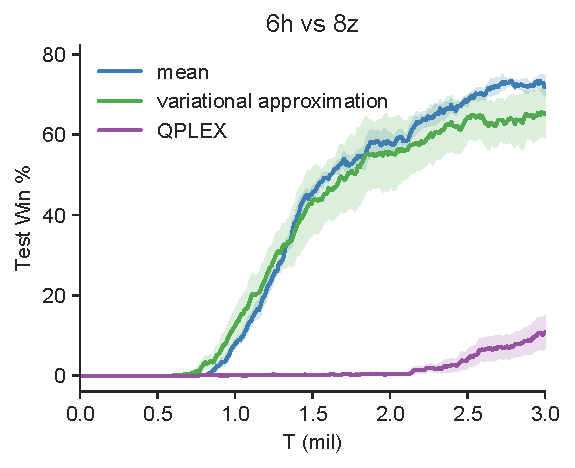
\includegraphics[width=0.9\linewidth]{pic/ab_bahavior.pdf}
	\caption{Comparison of assuming $p\left(i d | \tau_{t}\right) \approx p\left(i d\right)$ and estimating $p\left(i d | \tau_{t}\right)$ with variational inference on a SMAC super hard map $\mathtt{6h\_vs\_8z}$.}
	\label{fig:compare_behavior}
\end{wrapfigure}

where $n$ is the number of agents.

However, in this paper, we encourage each agent to behave differently from others when necessary. As a result, it is likely that $p\left(i d\right)$ might occasionally be different from $p\left(i d | \tau_{t}\right)$, which means the above assumption might not be valid all the time. 

As an alternative, we can leave out the assumption by using the Monte Carlo method (MC) for estimating the distribution $p\left(i d | \tau_{t}\right)$. In tabular cases, we count from samples to calculate the frequency $p\left(id | \tau_{t}\right) = \frac{N\left(id, \tau_{t}\right)}{N\left(\tau_{t}\right)}$, where $N(\cdot)$ is the time of visitation. However, MC becomes impractical in complex environments such as GRF and SMAC with long horizons and continuous spaces. For these complex cases, inspired by~\citet{wang2020influence}, we adopt variational inference to learn a distribution $q_{\xi}\left(id | \tau_{t}\right)$, parameterized by a neural network with parameters $\xi$, to estimate $p\left(id | \tau_{t}\right)$ by optimizing the evidence lower bound (ELBO). 

We empirically test these two estimation methods on a SMAC super hard map $\mathtt{6h\_vs\_8z}$ (Fig.~\ref{fig:compare_behavior}) (the observation-aware diversity is estimated with Eq.~\ref{final reward_forward}). The experimental results demonstrate that the two methods have similar performance but assuming $p\left(i d | \tau_{t}\right) \approx p\left(i d\right)$ outperforms estimating $p\left(i d | \tau_{t}\right)$ with variational approximation in both average performance and variance between random seeds. We hypothesize that the estimation error renders the variational inference approach unstable. Therefore, we decide to use Eq.~\ref{eq:mean} to estimate $p\left(a_{t} | \tau_{t}\right)$ in this paper.

%Based on the outstanding performance of estimating $p\left(id | \tau_{t}\right)$ with Eq.~\ref{eq:mean}, we decided to use this method.
% But, as discussed above, variational approximation might cause an improper lower bound in practice. To answer whether to estimate $p\left(id | \tau_{t}\right)$ with ELBO or assume $p\left(i d | \tau_{t}\right) \approx p\left(i d\right)$,
%At the beginning of training, the performance of variational approximation is slightly better. However, as training goes on, the variance between random seeds becomes more noticeable because of variational approximation error. Based on the outstanding performance of estimating $p\left(id | \tau_{t}\right)$ with Eq.~\ref{eq:mean}, we decided to use this method.


%Then, $p\left(a_{t} | \tau_{t}\right)$ is estimated by $\sum_{i d} q_{\xi}\left(i d | \tau_{t}\right) \pi\left(a_{t} | \tau_{t}, i d\right)$. With tractable $\pi\left(a_{t} | \tau_{t}, i d\right)$, the intractability of $p\left(a_{t} | \tau_{t}\right)$ has been reduced to a minimum.



%However, when the problem space becomes large, this Monte Carlo method (MC) consumes large memory in practice. Moreover, $\tau_t$ , which exponentially aggravates the tricky degree of MC on the largest scale of time steps. Inspired by EDTI~\cite{wang2020influence}, we can adopt variational inference to learn variational distributions $q_{\xi}\left(id | \tau_{t}\right)$, parameterized via neural networks with parameters $\xi$, by optimizing the evidence lower bound. Then, $p\left(a_{t} | \tau_{t}\right)$ is estimated by $\sum_{i d} q_{\xi}\left(i d | \tau_{t}\right) \pi\left(a_{t} | \tau_{t}, i d\right)$. With tractable $\pi\left(a_{t} | \tau_{t}, i d\right)$, the intractability of $p\left(a_{t} | \tau_{t}\right)$ has been reduced to a minimum.

%Fortunately, our novel policy representation structure can reduce this gap by sharing experience. In the extreme case, where the weight of L1 regularization term $\lambda \to \infty$, all agents' policies will be the same. So the assumption of $p\left(i d | \tau_{t}\right) \approx p\left(i d\right)$ is also reasonable in our paper. In this way, we have 

%\begin{equation}
%\begin{aligned} 
%p\left(a_{t} | \tau_{t}\right)
%&\approx \sum_{i d} p\left(i d\right) \operatorname{SoftMax}\left(Q_{\theta}\left(a_{t} | \tau_{t}, i d\right)\right) 
%\\ &= \frac{1}{N}\sum_{i d}  \operatorname{SoftMax}\left(Q_{\theta}\left(a_{t} | \tau_{t}, i d\right)\right).
%\end{aligned}
%\end{equation}


\subsection{Intrinsic Rewards for Observation-Aware Diversity}
We then analyze term \raisebox{.5pt}{\textcircled{\raisebox{-.9pt}{3}}}, which is related to observation-aware diversity. This part can be written as:
\begin{equation}
\begin{aligned} 
\raisebox{.5pt}{\textcircled{\raisebox{-.9pt}{3}}}=\sum_{t=0}^{T-1}E_{i d, \tau} \left[\log \frac{p(o_{t+1}| \tau_t,a_t,id)}{p(o_{t+1}| \tau_t,a_t)}\right].
\end{aligned}
\end{equation}
The computational problem here is how to estimate $p\left(o_{t+1} | \tau_{t}, a_{t}\right)$. We can directly adopt variational inference and learn the variational distribution $q_{\phi_2}\left(o_{t+1} | \tau_{t}, a_{t}\right)$, parameterized by a neural network with parameters $\phi_2$, by optimizing the evidence lower bound. With $q_{\phi_2}\left(o_{t+1} | \tau_{t}, a_{t}\right)$, $r^{I}$ can be written as:
\begin{equation}
\begin{aligned} 
r^I &=  E_{id}\left[\beta_2 D_{\mathrm{KL}}({\rm SoftMax}(\beta_1 Q(\cdot | \tau_t, id)) || p(\cdot| \tau_t)) \right.
\\& \left.+ \beta_1 \log q_{\phi}\left(o_{t+1} | \tau_{t}, a_{t}, i d\right)-\log q_{\phi_2}\left(o_{t+1} | \tau_{t}, a_{t}\right)\right].
\end{aligned}
\label{final reward_forward}
\end{equation}
This method use a \textbf{forward} prediction model of agents' next observation.

One concern is that the forward method involves inference on the continuous observation space, which may be too large to estimate accurately on complex tasks. We can omit it by deriving a lower bound.

We have that
%Unfortunately, any variational approximation will also cause an improper lower bound like which introduced in Eq.~\ref{eq:flaw1}:
%\begin{equation}
%\begin{aligned}
%r_{2, t}^I &= E_{i d}\left[\log q_{\phi}\left(o_{t+1} | \tau_{t}, a_{t}, i d\right)-\log q\left(o_{t+1} | \tau_{t}, a_{t}\right)\right]-D_{\mathrm{KL}}\left(p\left(o_{t+1} | \tau_{t}, a_{t}\right)  \| q\left(o_{t+1} | \tau_{t}, a_{t}\right)\right)
%\\ & \leq E_{i d}\left[\log q_{\phi}\left(o_{t+1} | \tau_{t}, a_{t}, i d\right)-\log q\left(o_{t+1} | \tau_{t}, a_{t}\right)\right],
%\end{aligned}
%\end{equation}
%which means any $q\left(o_{t+1} | \tau_{t}, a_{t}\right)$ used to estimate $r_{2, t}^{I}$ will lead to an overestimation and might cause our information-theoretic objective not being optimized correctly.
\begin{equation}
E[\log p(o' | \tau, a, id) - \log p(o' | \tau, a)] = I(o'; id | \tau, a).
\end{equation}
Therefore, optimising term \raisebox{.5pt}{\textcircled{\raisebox{-.9pt}{3}}} is equivalent to optimising $I(o'; id | \tau, a)$. Notice that
\begin{equation}
    I(o'; id | \tau, a) = H(o' | \tau, a) - H(o' | \tau, a, id), 
\end{equation}
we have 
\begin{equation}
\begin{aligned} 
I(o'; id | \tau, a) &=-H\left(o^{\prime} | \tau, a, id\right)+H\left(o^{\prime} | \tau, a\right) 
\\ &= -H\left(o^{\prime} | \tau, a, id\right)+ \sum_{o^{\prime}, \tau, a}p(o^{\prime}, \tau, a)\log \frac{p(\tau, a)}{p(o^{\prime}, \tau, a)}
\\ &= -H\left(o^{\prime} | \tau, a, id\right)+\sum_{o^{\prime}, \tau, a}p(o^{\prime}, \tau, a)\log \sum_{id} q\left(id | o^{\prime}, \tau, a\right)\frac{p(\tau, a)}{p(o^{\prime}, \tau, a)}
\\ &= -H\left(o^{\prime} | \tau, a, id\right)+\sum_{o^{\prime}, \tau, a}p(o^{\prime}, \tau, a)\log \sum_{id} q\left(id | o^{\prime}, \tau, a\right)\frac{p(id|o^{\prime}, \tau, a)p(\tau, a)}{p(o^{\prime}, id, \tau, a)}
\\ & \geq -H\left(o^{\prime} | \tau, a, id\right)+\sum_{o^{\prime}, \tau, a}p(o^{\prime}, \tau, a)\sum_{id} p\left(id | o^{\prime}, \tau, a\right)\log \frac{q(id|o^{\prime}, \tau, a)p(\tau, a)}{p(o^{\prime}, id, \tau, a)}
\\ & = -H\left(o^{\prime} | \tau, a, id\right)+\sum_{o^{\prime}, id, \tau, a}p(o^{\prime}, id, \tau, a)\log \frac{q(id|o^{\prime}, \tau, a)}{p(o^{\prime}, id| \tau, a)}
\\ & = -H\left(o^{\prime} | \tau, a, id\right)+E\left[\log q\left(id | o^{\prime}, \tau, a\right)\right]+H\left(o^{\prime}, id | \tau, a\right),
\end{aligned}
\label{eq:elbo_r2}
\end{equation}
where $q(id|o^{\prime}, \tau, a)$ can be an arbitrary distribution. We use variational inference and a neural network parameterized by $\eta_1$ to estimate it. Moreover, $H\left(o^{\prime}, i d | \tau, a\right)$ can be decomposed as:
% the distribution of agents' identity $q_{\eta_1}\left(i d | o^{\prime}, \tau, a\right)$
%we use the inequality for $H\left(o^{\prime} | \tau, a\right)$ to introduce an variational lower bound, with the variational posterior for agents' identity inference $q_{\eta_1}\left(i d | o^{\prime}, \tau, a\right)$. Moreover, $H\left(o^{\prime}, i d | \tau, a\right)$ can be decomposed as:
% , by optimizing $D_{\mathrm{KL}}(p(\cdot | o^{\prime}, \tau, a) \| q_{\eta_1}(\cdot | o^{\prime}, \tau, a))$ to reduce the inequality gap.
\begin{equation}
H\left(o^{\prime}, id | \tau, a\right)=H(id | \tau, a)+H\left(o^{\prime}| \tau, a, id \right).
\label{eq:entropy_decompose}
\end{equation}
With Eq.~\ref{eq:entropy_decompose}, Eq~\ref{eq:elbo_r2} can be further written as:
\begin{equation}
\begin{aligned} 
I(o'; id | \tau, a) & \geq -H\left(o^{\prime} | \tau, a, id\right)+E\left[\log q_{\eta_1}\left(id | o^{\prime}, \tau, a\right)\right]+H\left(o^{\prime}, id | \tau, a\right)
\\ &= -H\left(o^{\prime} | \tau, a, id\right) + E\left[\log q_{\eta_1}\left(id | o^{\prime}, \tau, a\right)\right]+H(id | \tau, a) + H\left(o^{\prime} | \tau, a, id\right)
\\ &= E\left[\log q_{\eta_1}\left(id | o^{\prime}, \tau, a\right)\right]+H(id | \tau, a)
\\ &= E\left[\log q_{\eta_1}\left(id | o^{\prime}, \tau, a\right) - \log p(id | \tau, a)\right].
\end{aligned}
\label{eq:r2_end}
\end{equation}
With the above mathematical derivation, we bypass the estimation of $p\left(o_{t+1} | \tau_{t}, a_{t}\right)$. Although $p(id | \tau_t, a_t)$ is introduced, we now infer in a much smaller and discrete space rather than the continuous observation space. We can estimate $p(id | \tau_t, a_t)$ using similar methods introduced in the previous section. We adopt variational inference to learn the distribution $q_{\eta_2}\left(i d | \tau_{t}, a_t\right)$, parameterized by a neural network with parameters $\eta_2$, by optimizing the evidence lower bound. With this \textbf{backward} prediction model of agents' identity, $r^I$ can be written as:
%However, any variational approximation for $p(i d | \tau, a)$ might again result in an improper lower bound for $I^{\boldsymbol{\pi}}\left(\tau_{T} ; i d\right)$.
\begin{equation}
\begin{aligned} 
r^I &=  E_{id}\left[\beta_2 D_{\mathrm{KL}}({\rm SoftMax}(\beta_1 Q(\cdot | \tau_t, id)) || p(\cdot| \tau_t)) \right.
\\& \left.+ \beta_1 \log q_{\eta_1}\left(id | o_{t+1}, \tau_t, a_t\right)-\log q_{\eta_2}\left(i d | \tau_{t}, a_t\right)\right].
\end{aligned}
\label{final reward_back}
\end{equation}

\begin{wrapfigure}[16]{r}{0.5\linewidth}
	\centering
	\vspace{-0.6cm}
	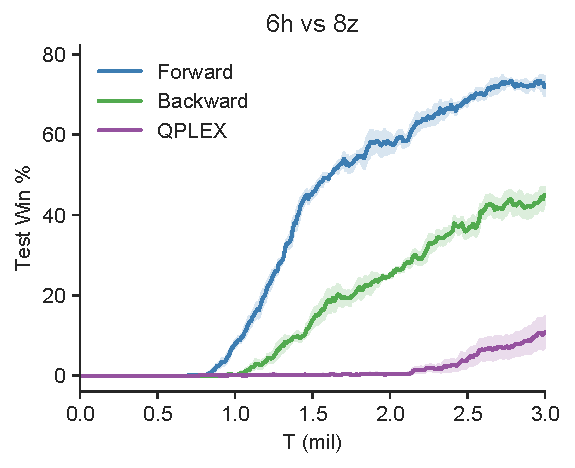
\includegraphics[width=0.9\linewidth]{pic/ab_6h8z.pdf}
	\caption{Comparison of forward and backward estimation for observation-aware diversity on a SMAC super hard map $\mathtt{6h\_vs\_8z}$.}
	\label{fig:compare_trans}
\end{wrapfigure}
We empirically compare these two methods on a SMAC super hard map $\mathtt{6h\_vs\_8z}$ as shown in Fig.~\ref{fig:compare_trans} ($p(\cdot| \tau_t)$ is estimated with Eq.~\ref{eq:mean}). The experimental results demonstrate that estimating $r^{I}$ with a forward prediction model noticeably outperforms estimating with a backward prediction model, although the forward model might be more difficult to estimate as discussed before. We hypothesize that simultaneously and independently estimating $q_{\phi}\left(o_{t+1} | \tau_{t}, a_{t}, i d\right)$ and $q_{\phi_2}\left(o_{t+1} | \tau_{t}, a_{t}\right)$ might bring advantages similar to those of curiosity-driven methods, leading to outstanding performance on tasks requiring extensive exploration, so we use Eq.~\ref{final reward_forward} to encourage diversity in this paper. 
% We hypothesize that this is because the variational posterior for agents' identity $q_{\eta_1}\left(i d | o^{\prime}, \tau, a\right)$ is easier to estimate than $q_{\phi}\left(o_{t+1} | \tau_{t}, a_{t}, i d\right)$, which infers in the continuous observation space rather than in the discrete identification space of the size of the number of agents. 
%Here we further discuss the relationship of our approach and EOI~\cite{jiang2020emergence}. For intrinsic rewards, EOI optimizes $I(id ; o)$ by maximizing $p(id|o)$. Our approach optimizes $I(\tau_T ; id)$ with intrinsic rewards by splitting it as action-aware diversity and observation-aware diversity. In structure, EOI introduces intrinsic value function (IVF) to estimate the discounted sum of $p(id|o)$. Then, EOI combines the gradient from IVF and $Q_{tot}$ to train each agent's local Q-function. However, in the multi-agent setting, agents' observations can be influenced by other agents. Therefore, $p(id|o)$ is determined by the behaviors of all agents. Moreover, the direct combination of gradient means each agent equally treats identity and the completion of tasks, but which are not equivalent in most tasks, which increases the difficulty in optimizing EOI. The two problems discussed above are the main reason forbidding EOI to be applied in more challenging and complex tasks. As for our approach, these problems do not exist. Our approach encourages agents to highlight themselves from others in behavior and next observation with identity-aware diversity. We realize that our diversity-encouraging reward inevitably involves the influence of all agents. So we combine our intrinsic reward with environmental rewards to train the total Q-function, which is a combination of individual Q-functions. In this way, the centralized trainer will consider balancing diversity and tasks by leading diversity to a more valuable form, beneficial to tasks. Further, we consider the shared local Q-functions do not have enough capacity to represent diversity. Then, we decomposed individual Q-functions as the sum of shared and non-shared local Q-functions for taking the merits of sharing parameters while maintaining representation diversity.
%We specifically describe the impact from other agents with observation-aware diversity and encourage agents to behave differently with action-aware diversity.
%EOI only considers encouraging agents to have different observations. Our approach further considers other agents' impact while optimizing observation-aware diversity and encourages agents to make different actions for action-aware diversity. 

%In multiagent setting, agents have impact with each other, which means next observation cannot be excatly predicted after knowing ego agent's trajectory and action.


%Here we further discuss the relationship of our approach and EOI~\cite{jiang2020emergence}. EOI introduces intrinsic value functions (IVF) to estimate the discounted sum of $p(id | o)$ with TD loss. With the chain rule, individual local Q-functions are updated with the combination of (1) the TD error of $Q^{\text {tot }}$ for completing the joint task, and (2) the gradient backpropagated from IVF for diversity. It is a good idea to consider diversity and the accomplishment of joint tasks at the same time. However, the direct combination of gradients optimizing different targets is perilous. In particular, we are considering how to let agents achieve sophisticated strategies for cooperation. The sudden change of any agent might cause all previous training to fail because of the break of coordination. Two main components of our approach, identity-aware diversity and partially shared networks with L1 regularization, can be seen as 


\section{Experiment Details}

\subsection{Baselines}\label{Baselines}

We compare our approach with multi-agent value-based methods (QMIX~\cite{rashid2018qmix} \& QPLEX~\cite{wang2020qplex}), a variational exploration method (MAVEN~\cite{mahajan2019maven}), and an individuality emergence (EOI~\cite{jiang2020emergence}) method. For QMIX, QPLEX, MAVEN, and EOI, we use the codes provided by the authors, whose hyper-parameters have been fine-tuned.
% We firmly believe the published codes are correctly used.

\subsection{Architecture and Hyperparameters}\label{sec:hyper}

In this paper, we use a QPLEX style mixing network with its default hyperparameters suggested by the original paper. Specifically, in complex environments (GRF and SMAC), the transformation part has four 32-bits attentional heads, each with one middle layer of 64 units. Weights in the joint advantage function of the dueling mixing part are produced by a four-head attention module without hidden layers. In toy environment $\mathtt{Pac}$-$\mathtt{Men}$, we do not use the transformation part but still generate weights in the joint advantage function of the dueling mixing part by the four-head module without hidden layers. For individual Q-functions, agents share a trajectory encoding network consisting of two layers, a fully connected layer followed by a GRU layer with a 64-dimensional hidden state. After the trajectory encoding network, all agents share a one-layer Q network, while each agent has its independent Q network with the same structure as the shared Q network. 

For all experiments, the optimization is conducted using RMSprop with a learning rate of $5 \times 10^{-4}$, $\alpha$ of 0.99, and with no momentum or weight decay. For exploration, we use $\epsilon$-greedy, with $\epsilon$ annealed linearly from $1.0$ to $0.05$ over $500K$ time steps and kept constant for the rest of the training, for both CDS and all the baselines and ablations. Our method introduces four important hyperparameters: $\beta$, $\beta_1$, $\beta_2$, that are related to the intrinsic rewards, and $\lambda$, which is the scaling weight of the L1 regularization term. For the environment in the case study ($\mathtt{Pac}$-$\mathtt{Men}$), $\lambda$ is set to 0.01. For GRF and SMAC, we set $\lambda$ to 0.1 to strengthen \emph{being diverse only when necessary}. For other hyperparameters related to intrinsic rewards, we tune with grid search ($\beta \in\{0.05,0.1,0.2\}, \beta_{1} \in\{0.5,1.0,2.0\}, \text { and } \beta_{2} \in\{0.5,1.0,2.0\}$). We tune for GRF on the $\mathtt{academy\_3\_vs\_1\_with\_keeper}$. We notice $\mathtt{Corridor}$ has a fundamental difference compared with $\mathtt{6h\_vs\_8z}$, $\mathtt{MMM2}$ and $\mathtt{3s5z\_vs\_3s6z}$ in the ratio of the number of enemy agents to our agents, which requires different kinds of sophisticated strategies. Our approach can be compatible with different situations by adjusting the ratio of $H\left(\tau_{T}\right)$ and $H\left(\tau_{T} \mid i d\right)$ in Eq.~\ref{equ:mutual_information}. So we tune hyperparameters for SMAC on both $\mathtt{6h\_vs\_8z}$ and $\mathtt{Corridor}$. For other SMAC maps, we fine-tune $\beta$ to get better adaptability to the environments. Moreover, for GRF scenarios, we use a prioritized replay buffer of the TD error for CDS, all the baselines, and ablations.

\begin{table}[h]
%\begin{wraptable}[15]{r}{0.5\linewidth}
\centering
\caption{CDS Hyperparameters.}
\begin{tabular}{lllllll}
\hline                  & Environment                                       & $\beta$      & $\beta_1$ & $\beta_2$ & $\lambda$
\\ \hline Case Study    & $\mathtt{Pac}$-$\mathtt{Men}$                     & 0.15         & 2.0       & 1.0       & 0.01
\\ \hline               & $\mathtt{6h\_vs\_8z}$                             & 0.1          & 2.0       & 1.0       & 0.1
\\                      & $\mathtt{MMM2}$                                   & 0.07         & 2.0       & 1.0       & 0.1
\\                      & $\mathtt{3s5z\_vs\_3s6z}$                         & 0.03         & 2.0       & 1.0       & 0.1
\\ SMAC                 & $\mathtt{Corridor}$                               & 0.1          & 0.5       & 0.5       & 0.1
\\                      & $\mathtt{3s\_vs\_5z}$                             & 0.04         & 0.5       & 0.5       & 0.1
\\                      & $\mathtt{5m\_vs\_6m}$                             & 0.01         & 2.0       & 1.0       & 0.1
\\ \hline               & $\mathtt{academy\_3\_vs\_1\_with\_keeper}$        & 0.1          & 0.5       & 1.0       & 0.1
\\ GRF                  & $\mathtt{academy\_counterattack\_hard}$           & 0.1          & 0.5       & 1.0       & 0.1
\\                      & $\mathtt{3\_vs\_1\_with\_keeper\ (full\ field)}$  & 0.1          & 0.5       & 1.0       & 0.1
\\ \hline
\label{table_baseline}
\end{tabular}
%\end{wraptable}
\end{table}

%\begin{table}[h]
%\newcounter{2} 
%\setcounter{2}{\value{table}} % 将当前序号 赋给TempEqCnt
%\setcounter{table}{1}  
%\caption{Hyperparameters}
%\centering
%\begin{tabular}{llllll}
%\hline & \makecell{Environment} & \makecell{$\beta$} & \makecell{$\beta_1$} & \makecell{$\beta_2$} & \makecell{$\lambda$}
%\\ \hline & \makecell{$\mathtt{Pac}$-$\mathtt{Men}$ (case study)} & \makecell{0.15} & \makecell{2.0} & \makecell{1.0} & \makecell{0.01}
%\\  \hline & \makecell{$\mathtt{academy\_3\_vs\_1\_with\_keeper}$(GRF)} & \makecell{0.05} & \makecell{0.5} & \makecell{2.0} & \makecell{0.1}
%\\  & \makecell{$\mathtt{academy\_counterattack\_hard}$(GRF)} & \makecell{0.05} & \makecell{0.5} & \makecell{2.0} & \makecell{0.1}
%\\  & \makecell{$\mathtt{3\_vs\_1\_with\_keeper (full\ field)}$(GRF)} & \makecell{0.05} & \makecell{0.5} & \makecell{2.0} & \makecell{0.1}
%\\  \hline & \makecell{$\mathtt{corridor}$ (SMAC)} & \makecell{0.1} & \makecell{2.0} & \makecell{1.0} & \makecell{0.1}
%\\  & \makecell{$\mathtt{MMM2}$ (SMAC)} & \makecell{0.07} & \makecell{2.0} & \makecell{1.0} & \makecell{0.1}
%\\  & \makecell{$\mathtt{6h vs 8z}$ (SMAC)} & \makecell{0.1} & \makecell{2.0} & \makecell{1.0} & \makecell{0.1}
%\\  & \makecell{$\mathtt{3s5z vs 3s6z}$ (SMAC)} & \makecell{0.03} & \makecell{2.0} & \makecell{1.0} & \makecell{0.1}
%\\ \hline
%\label{table2}
%\end{tabular}
%\end{table}

%we first fix $\beta=0.1$ and $\lambda=0.1$, then search best hyperparameters for $\beta_1$ and $\beta_2$ in the set $\{0.5, 1.0, 2.0\}$. After that, we first search $\lambda=0.01$, then search $\beta$ in the set $\{0.05, 0.1, 0.15, 0.2\}$. For GRF scenarios, we only search hyperparameters on $\mathtt{academy\_3\_vs\_1\_with\_keeper}$. We first fix $\beta=0.1$ and $\lambda=0.1$ and search best hyperparameters for $\beta_1$ and $\beta_2$ in the set $\{0.5, 1.0, 2.0\}$. After that, we search $\beta$ in the set $\{0.05, 0.1, 0.15, 0.2\}$. For SMAC benchmarking tasks, we only search $\beta_1$ and $\beta_2$ in $\mathtt{corridor}$ in the set $\{0.5, 1.0, 2.0\}$. But we find $\beta$ is sensitive in different tasks. So we search $\beta$ in $[0.01, 0.1]$ for each task.



\subsection{GRF Scenarios}
\label{sec:grf_scen}
\begin{figure*}[ht]
\centering
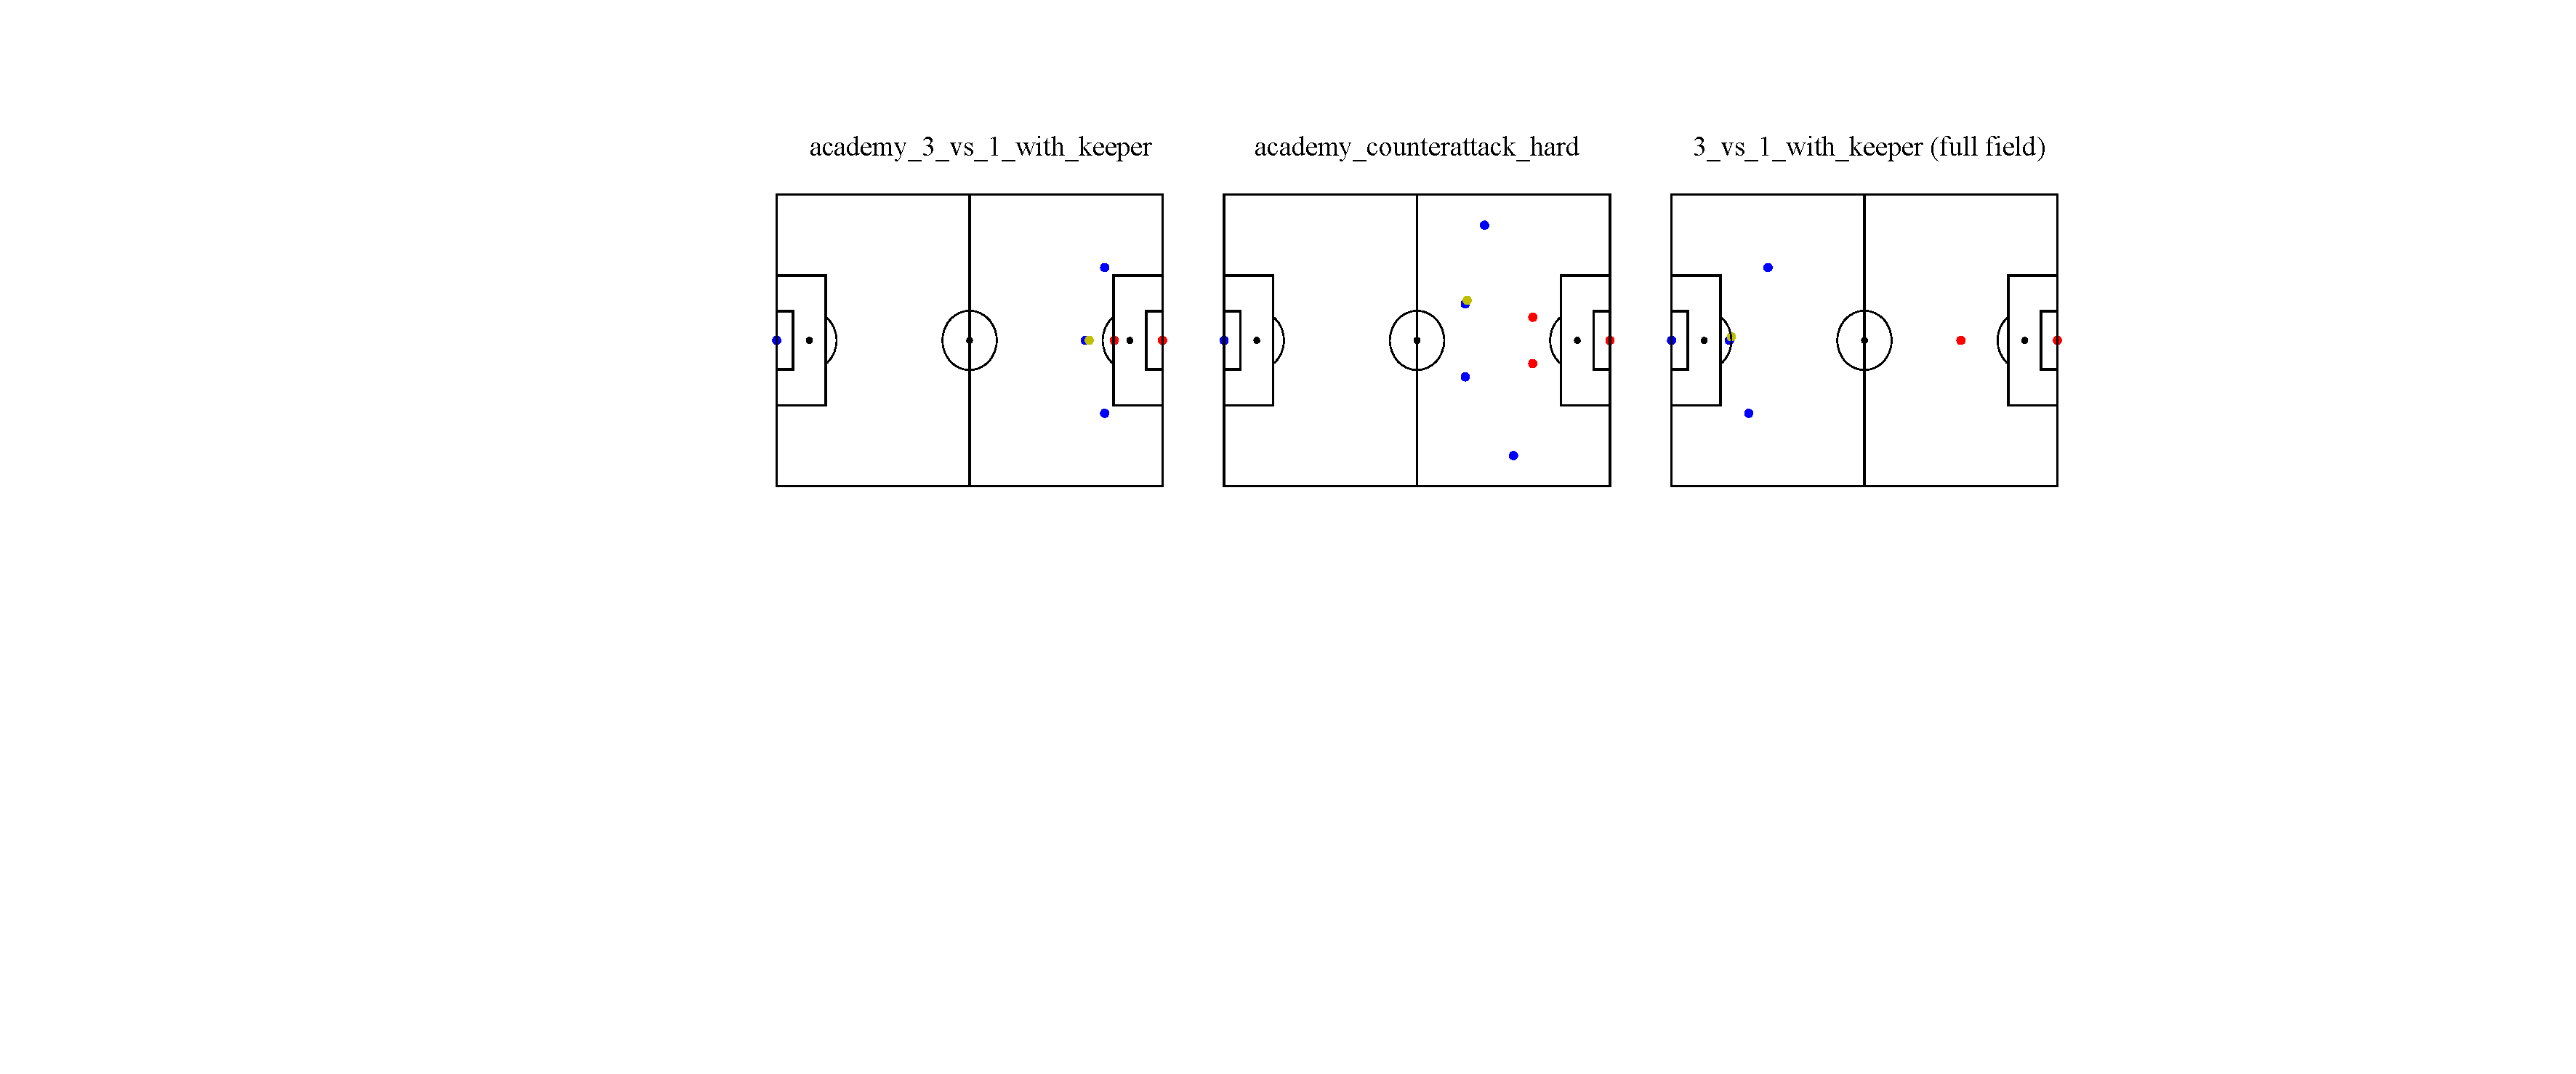
\includegraphics[width=1.\linewidth]{pic/env_football.pdf}
\caption{Visualization of the initial position of each agent in three GRF environments considered in our paper, where blue points represent our agents, red points represent opponents, and the yellow point represents the ball.}
\label{grf_initial}
\end{figure*}

In this paper, we achieve state-of-the-art performance on all the tested GRF tasks, including two official scenarios $\mathtt{academy\_3\_vs\_1\_with\_keeper}$ and $\mathtt{academy\_counterattack\_hard}$. Furthermore, we design one full-field scenario $\mathtt{3\_vs\_1\_with\_keeper\ (full\ field)}$ to compare the performance of our approach and baselines on a task with a more complex problem space. The visualization of the initial position of each agent for the three GRF scenarios are shown in Fig.~\ref{grf_initial}.

\subsection{Infrastructure}
\label{sec:gtx}

Experiments are carried out on NVIDIA GTX 2080 Ti GPU. And the training of our approach on all environments can be finished in less than two days.

%\section{Additional Experimental Results}

%\subsection{More Experiments on Pac-Men}

%\begin{figure}[h]
%	\centering
%    \includegraphics[height=0.32\linewidth]{pic/pacmen_EDTI.pdf}
%    \includegraphics[height=0.32\linewidth]{pic/pacmen_EITI.pdf}
%	\caption{Comparison against EDTI and EITI with partial network sharing on $\mathtt{Pac}$-$\mathtt{Men}$.}
%	\label{fig:EDTI_EITI_more}
%\end{figure}

%In Sec. ~\ref{sec:how_work}, we show that our approach outperforms baselines in a toy game $\mathtt{Pac}$-$\mathtt{Men}$, where EDTI or EITI is combined with a current state-of-the-art multi-agent factored Q-learning algorithm QPLEX. In this section, we further test EDTI and EITI augmented by the \name~novelties (agents share a local Q-function, and each has an individual Q-function regularized by the L1 loss). As shown in Fig.~\ref{fig:EDTI_EITI_more}, with more diversity capacity provided by \name, EDTI and EITI achieve better performance, but still underperform our method. These results indicate that (1) our structural contribution that enables agents to have exclusive knowledge is readily to be combined with other MARL methods and is likely to improve their performance; (2) our learning objective is more efficient on tasks that require diversity among agents.


%\subsection{More Experiments on Google Research Football}

%\begin{figure*}[ht]
%\centering
%\includegraphics[width=1.\linewidth]{pic/ab_EDTI_grf.pdf}
%\caption{Comparison against EDTI with partial network sharing on GRF.}
%\label{fig:GRF_EDTI}
%\end{figure*}

%\begin{figure*}[ht]
%\centering
%\includegraphics[width=1.\linewidth]{pic/ab_EITI_grf.pdf}
%\caption{Comparison against EITI with partial network sharing on GRF.}
%\label{fig:GRF_EITI}
%\end{figure*}

%In this section, we further test EDTI and EITI augmented by \name~innovations on Google Research Football. As shown in Fig.~\ref{fig:GRF_EDTI} and~\ref{fig:GRF_EITI}, augmented EDIT and EITI perform noticeably better in complex Football scenarios, demonstrating the power of our neural network structures shown in Fig.~\ref{fig:model}. Moreover, our diversity learning objective still outperforms EDTI and EITI, showing its efficiency in challenging multi-agent tasks.

%\subsection{Advantages and Limitations of Our Approach}

%In this paper, we achieve \emph{being diverse when necessary} with the combination of structural and motivational novelties. Our approach pushes forward the state of the art on challenging GRF scenarios and significantly outperforms baselines on three super hard maps from the SMAC benchmark. Our approach encourages each agent to highlight itself from the group and balance this diversity with sharing to learn sophisticated strategies. But when facing larger problem spaces, this balancing process will require more training. Further, we only maintain one shared neural network among agents. The representational capacity might not be enough when dealing with more complex tasks that require multiple types of shared behaviors, such as learning offense and defense at the same time. We plan to explore how to improve our approach's scalability and representational ability for the GRF full game in future works.

% other than local Q-functions whose usage are limited by L1 regularization terms
%in current challenging MARL tasks, such as GRF and SMAC,  
%Our approach optimizes $I(\tau_T ; id)$ with intrinsic rewards by splitting it as action-aware diversity and observation-aware diversity. We realize that our diversity-encouraging reward inevitably involves the influence of all agents. So we combine our intrinsic reward with environmental rewards to train the total Q-function, which is a combination of individual Q-functions. In this way, the centralized trainer will consider balancing diversity and tasks by leading diversity to a more valuable form, beneficial to tasks. Further, we consider the shared local Q-functions do not have enough capacity to represent diversity. Then, we decomposed individual Q-functions as the sum of shared and non-shared local Q-functions for taking the merits of sharing parameters while maintaining representation diversity.